\section{Chemical Kinetics, Equilibrium and Energetics}

\begin{multicols}{2}


\section*{Rate of Chemical Reactions}


\subsection[Effect of Temperature on Reaction Rate]{Effect of Temperature on \hfill \\ Reaction Rate}

%\begin{center}
%\includegraphics[width=0.4\textwidth]{./img/.jpg}
%\end{center}

\begin{description*}
%\item[Subtopic:]{}
\item[Materials:]{4 syringes, \nameref{sec:test-tube-racks}, vinegar, baking soda, water \nameref{sec:heatsources}}
\item[Setup:]{Prepare a solution of sodium hydrogen carbonate (baking soda) by dissolving about 3 teaspoons per litre of water.}
\item[Procedure:]{Arrange 4 syringe test tubes in the rack and label them 1, 2, 3 and 4. Add about 3 mL of acid to tubes 1 and 2. Add 3 mL of base to tubes 3 and 4. Heat tubes 2 and 4 in the boiling water bath until they are near boiling. Pour tube 3 into tube 1, and pour tube 4 into tube 2.}
%\item[Hazards:]{}
%\item[Questions:]{}
\item[Observations:]{The reaction between tubes 2 and 4 produces bubbles much faster than the reaction between tubes 1 and 3.}
\item[Theory:]{The rate of a chemical reaction increases with an increase in temperature.}
%\item[Applications:]{}
%\item[Notes:]{}
\end{description*}

\subsection[Effect of Concentration on Reaction Rate]{Effect of Concentration on \hfill \\ Reaction Rate}
% PIC!!! syringes stuck in bottles

%\begin{center}
%\includegraphics[width=0.4\textwidth]{./img/.png}
%\end{center}

\begin{description*}
%\item[Subtopic:]{}
\item[Materials:]{3 bottles, 3 syringes, baking soda, vinegar, nail, super glue}
\item[Setup:]{Poke a hole through the lids of 3 bottles using a heated nail. Insert the tip of a 20 mL syringe in each and seal with super glue.}
\item[Procedure:]{Add 4, 2 and 1 teaspoons of baking soda to each of the 3 bottles respectively. Dilute each to 20 mL using water. Put 10 mL of vinegar in the first syringe, 5 mL in the second, and 2.5 mL in the third. Dilute each to 20 mL using water. Screw on each cap to its corresponding bottle and empty all 3 syringes at once.}
%\item[Hazards:]{}
%\item[Questions:]{}
\item[Observations:]{As the reaction proceeds, the syringes are pushed upward. The first syringe is pushed up first, followed by the second and then the third.}
\item[Theory:]{The combination of baking soda (bicarbonate of soda) and vinegar produces carbon dioxide as a product, which pushes the syringe plunger upwards and fills the syringe. The higher the concentration of the reactants, the faster the reaction will proceed.}
%\item[Applications:]{}
%\item[Notes:]{}
\end{description*}

\columnbreak

\subsection[Effect of Surface Area on Reaction Rate]{Effect of Surface Area on \hfill \\ Reaction Rate}

%\begin{center}
%\includegraphics[width=0.4\textwidth]{./img/.jpg}
%\end{center}

\begin{description*}
%\item[Subtopic:]{}
\item[Materials:]{2 syringes/bottles, dilute sulphuric acid, iron nail, iron wool}
%\item[Setup:]{}
\item[Procedure:]{Add small but equal amounts of dilute sulphuric acid to each container. In one, place an iron nail. In the other, place a piece of iron wool.}
\item[Hazards:]{Dilute sulphuric acid is corrosive to the skin and clothes and can cause
damage to the eyes. Neutralize spills with baking soda.}
%\item[Questions:]{}
\item[Observations:]{Bubbles of hydrogen gas should be observed on the
iron in both containers. The rate of bubble formation, however, should be much faster on
the steel wool. After a minute, the difference in the rate of reaction
should be observed.}
\item[Theory:]{The bubbles form much more quickly from the steel
wool than from the iron nail because it has a much higher surface area.}
%\item[Applications:]{}
%\item[Notes:]{}
\end{description*}

\subsection[Effect of a Catalyst on Reaction Rate]{Effect of a Catalyst on \hfill \\ Reaction Rate}

%\begin{center}
%\includegraphics[width=0.4\textwidth]{./img/.jpg}
%\end{center}

\begin{description*}
%\item[Subtopic:]{}
\item[Materials:]{Old dry cell, hydrogen peroxide, 2 bottles, 2 balloons}
\item[Setup:]{Remove the dark powder (manganese dioxide) from an old dry cell.}
\item[Procedure:]{Add a small amount of hydrogen peroxide to each bottle. Add the manganese dioxide powder to one and then cover both bottles with balloons.}
%\item[Hazards:]{}
%\item[Questions:]{}
\item[Observations:]{The balloon on the bottle containing manganese dioxide inflates, while the other does not.}
\item[Theory:]{Hydrogen peroxide decomposes very slowly at room temperature in to water and oxygen gas. The manganese (IV) oxide from the battery \emph{catalyzes} this reaction (speeds it up). Hence there is a notable change in the size of the balloon. The manganese (IV) oxide acts as a catalyst only by speeding up the reaction, not by increasing the amount of products formed.}
%\item[Applications:]{}
\item[Notes:]{The manganese dioxide does not get used up in this reaction. It can be dried and used again.}
\end{description*}

\columnbreak

\subsection[Organic and Inorganic Catalysts]{Organic and Inorganic \hfill \\ Catalysts} % Shika 294

%\begin{center}
%\includegraphics[width=0.4\textwidth]{./img/.jpg}
%\end{center}

\begin{description*}
%\item[Subtopic:]{}
\item[Materials:]{Old dry cell, hydrogen peroxide, 4 syringes, water, yeast, \nameref{sec:heatsources}, 4 balloons}
\item[Setup:]{Remove the dark powder (manganese dioxide) from an old dry cell.}
\item[Procedure:]{Add 5 mL of water to each syringe and label them 1, 2, 3 and 4. Add yeast to tubes 1 and 2. Add manganese dioxide to tubes 3 and 4. Heat tubes 2 and 4 in a hot water bath until they boil. Add 5 mL of hydrogen peroxide to each tube simultaneously and quickly cap them with balloons.}
%\item[Hazards:]{}
%\item[Questions:]{}
\item[Observations:]{Tube 4 inflates most quickly, while tube 2 does not inflate or does very little. Tubes 1 and 3 inflate at a slower rate.}
\item[Theory:]{Both catalase from yeast and manganese (IV) oxide from batteries act as catalysts. Catalase is a biological catalyst, while manganese (IV) oxide is not. Boiling the yeast in tube 2 destroys its catalase and hence slows down the reaction. Heating does not hinder the manganese dioxide, but in fact speeds up the reaction (tube 4). Tubes 1 and 3 still catalyze the reaction. }
\item[Applications:]{}
\item[Notes:]{Biological catalysts are subject to variations in the environment that kill or destroy biological activity.}
\end{description*}

%==================================================================================================%

\section*{Reversible and Irreversible \hfill \\ Reactions}


\subsection{Reversible Chemical Reaction}

%\begin{center}
%\includegraphics[width=0.4\textwidth]{./img/.jpg}
%\end{center}

\begin{description*}
%\item[Subtopic:]{}
\item[Materials:]{Copper (II) sulphate, spoon, \nameref{sec:heatsources}, water}
\item[Setup:]{Grind the copper (II) sulphate crystals into powder.}
\item[Procedure:]{Add a small amount of copper (II) sulphate to a metal spoon and heat gently over the heat source. Stop heating when the crystals have changed from blue to white. Let the spoon cool, and add a couple drops of water to the white crystals.}
%\item[Hazards:]{}
%\item[Questions:]{}
\item[Observations:]{The crystals regain their blue colour upon addition of water.}
\item[Theory:]{Heating the copper (II) sulphate changes it from blue (\ce CuSO4 $\cdot$ 5H2O) to white (\ce CuSO4). Adding water reverses this reaction and returns the crystals to their original hydrated state (blue).}
%\item[Applications:]{}
%\item[Notes:]{}
\end{description*}

\columnbreak

%==================================================================================================%

\section*{Endothermic and Exothermic Reactions}


\subsection{Temperature Bottles} % Moved to Fuels and Energy

\begin{center}
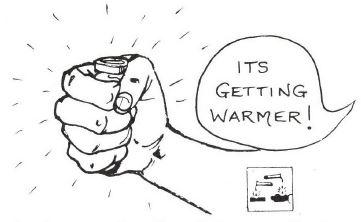
\includegraphics[width=0.4\textwidth]{./img/source/exothermic.jpg}
\end{center}

\begin{description*}
%\item[Subtopic:]{}
\item[Materials:]{3 plastic bottles, powdered soap, citric acid, spoon}
%\item[Setup:]{}
\item[Procedure:]{Add a small amount of water to each bottle. Add 3 spoons of powdered laundry soap (e.g. Omo, Foma) to the first bottle. Add 3 spoons of citric acid to the second bottle and nothing to the third bottle. Shake each vigorously and feel to observe any changes in temperature.}
%\item[Hazards:]{}
%\item[Questions:]{}
%\item[Observations:]{}
\item[Theory:]{The dissolution of laundry soap in water is exothermic -- this bottle should
get warmer. The dissolution of citric acid is endothermic -- this bottle should get cooler.}
%\item[Applications:]{}
%\item[Notes:]{}
\end{description*}
%
%%\subsection{Endothermic Reactions}
%%
%%%\begin{center}
%%%\includegraphics[width=0.4\textwidth]{./img/.png}
%%%\end{center}
%%
%%\begin{description*}
%%%\item[Subtopic:]{}
%%\item[Materials:]{Ammonium nitrate, water, container, thermometer (optional)}
%%%\item[Setup:]{}
%%\item[Procedure:]{Add water to a container or beaker. Add a small amount of ammonium nitrate and stir gently. After all of the ammonium nitrate has dissolved, feel the container or read the thermometer. }
%%%\item[Hazards:]{}
%%%\item[Questions:]{}
%%\item[Observations:]{The container has cooled.}
%%\item[Theory:]{This is an example of an \emph{endothermic} reaction. The heat content of the products is greater than the heat contents of the reactants, so the extra energy required is absorbed from the water.}
%%%\item[Applications:]{}
%%%\item[Notes:]{}
%%\end{description*}
%%
%%\subsection{Exothermic Reactions}
%%
%%\begin{center}
%%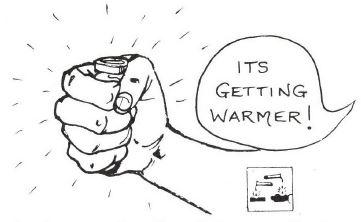
\includegraphics[width=0.4\textwidth]{./img/source/exothermic.jpg}
%%\end{center}
%%
%%\begin{description*}
%%%\item[Subtopic:]{}
%%\item[Materials:]{Battery acid, sodium hydroxide, bottle, thermometer (optional)}
%%%\item[Setup:]{}
%%\item[Procedure:]{Add a small amount of water to the container. Carefully pour a small amount of battery acid down the side of the container using a syringe or test tube. Gently stir and \emph{carefully} touch the side of the container or read the thermometer.}
%%\item[Hazards:]{The reaction between water and acid produces a lot of heat. Be extremely careful when touching the container. Do not use a highly concentrated acid and always wear goggles.}
%%%\item[Questions:]{}
%%\item[Observations:]{The container becomes very warm.}
%%\item[Theory:]{This is an example of an \emph{exothermic} reaction. The total heat content of the reactants is greater than that of the products, so excess energy is lost to the water.}
%%%\item[Applications:]{}
%%%\item[Notes:]{}
%%\end{description*}


\end{multicols}

\pagebreak